
\documentclass[twoside,11pt]{homework}
\usepackage{graphicx}
\usepackage{listings}
\usepackage{color}
\usepackage{bm}
\newcommand{\vect}[1]{\boldsymbol{\mathbf{#1}}}
\definecolor{dkgreen}{rgb}{0,0.6,0}
\definecolor{gray}{rgb}{0.5,0.5,0.5}
\definecolor{mauve}{rgb}{0.58,0,0.82}
\lstset{ %
	language=R,                     % the language of the code
	basicstyle=\footnotesize,       % the size of the fonts that are used for the code
	numbers=left,                   % where to put the line-numbers
	numberstyle=\tiny\color{gray},  % the style that is used for the line-numbers
	stepnumber=1,                   % the step between two line-numbers. If it's 1, each line
	% will be numbered
	numbersep=5pt,                  % how far the line-numbers are from the code
	backgroundcolor=\color{white},  % choose the background color. You must add \usepackage{color}
	showspaces=false,               % show spaces adding particular underscores
	showstringspaces=false,         % underline spaces within strings
	showtabs=false,                 % show tabs within strings adding particular underscores
	frame=single,                   % adds a frame around the code
	rulecolor=\color{black},        % if not set, the frame-color may be changed on line-breaks within not-black text (e.g. commens (green here))
	tabsize=2,                      % sets default tabsize to 2 spaces
	captionpos=b,                   % sets the caption-position to bottom
	breaklines=true,                % sets automatic line breaking
	breakatwhitespace=false,        % sets if automatic breaks should only happen at whitespace
	title=\lstname,                 % show the filename of files included with \lstinputlisting;
	% also try caption instead of title
	keywordstyle=\color{blue},      % keyword style
	commentstyle=\color{dkgreen},   % comment style
	stringstyle=\color{mauve},      % string literal style
	escapeinside={\%*}{*)},         % if you want to add a comment within your code
	morekeywords={*,...},            % if you want to add more keywords to the set
	belowcaptionskip=0em,
	belowskip=0em
} 

\usepackage{etoolbox}
\makeatletter
\patchcmd{\@verbatim}
{\verbatim@font}
{\verbatim@font\footnotesize}
{}{}
\preto{\@verbatim}{\topsep=0pt \partopsep=0pt }
\makeatother

\coursename{COMS 4771 Machine Learning } % DON'T CHANGE THIS

\studname{Jun Hu}    % YOUR NAME GOES HERE
\studmail{jh3846@columbia.edu}% YOUR UNI GOES HERE
\hwNo{4}                   % THE HOMEWORK NUMBER GOES HERE
\collab{}   % THE UNI'S OF STUDENTS YOU DISCUSSED WITH

% Uncomment the next line if you want to use \includegraphics.\textbf{\textbf{\textbf{}}}
%\usepackage{graphicx}

\begin{document}
\maketitle

\section*{Problem 1}

\begin{enumerate}
\item[\textbf{(a)}] Generate the data set as:

\begin{lstlisting}
set.seed(23)
p = 40
n = 2500
x = matrix(rnorm(n*p), n, p)
b = rnorm(p)
b[5]=b[7]=b[11]=b[13]=b[17]=b[19]=b[29]=b[31]=b[37] = 0
e = rnorm(n)
y = x % * % b + e
\end{lstlisting}

\item[\textbf{(b)}] Split the data set as:

\begin{lstlisting}
train = sample(seq(n*0.7), n*0.7, replace=FALSE)
y.train = y[train,]
y.test = y[-train,]
x.train = x[train,]
x.test = x[-train,]
data.train = data.frame(y=y.train, x=x.train)
data.test = data.frame(y=y.test, x=x.test)
\end{lstlisting}

\item[\textbf{(c)}] Perform boosting on the training set, and predict on test set as:

\begin{lstlisting}
library(gbm)
set.seed(23)
pows = seq(-10, 0, 0.1)
lambdas = 10^pows
boost.test.err = rep(NA, length(lambdas))
for (i in 1:length(lambdas)) {
boost.data = gbm(y~., data=data.train, distribution="gaussian", n.trees=1000, shrinkage=lambdas[i])
pred.boost.test = predict(boost.data, data.test, n.trees=1000)
boost.test.err[i] = mean((pred.boost.test-y.test)^2)
}
\end{lstlisting}

\item[\textbf{(d)}] Produce the plot on corresponding test set MSE as:

\begin{lstlisting}
plot(lambdas, boost.test.err, type="b", col="red", lwd=2, xlab="Shrinkage Values", ylab="Test MSE")
\end{lstlisting}

The plot is:
\begin{center}
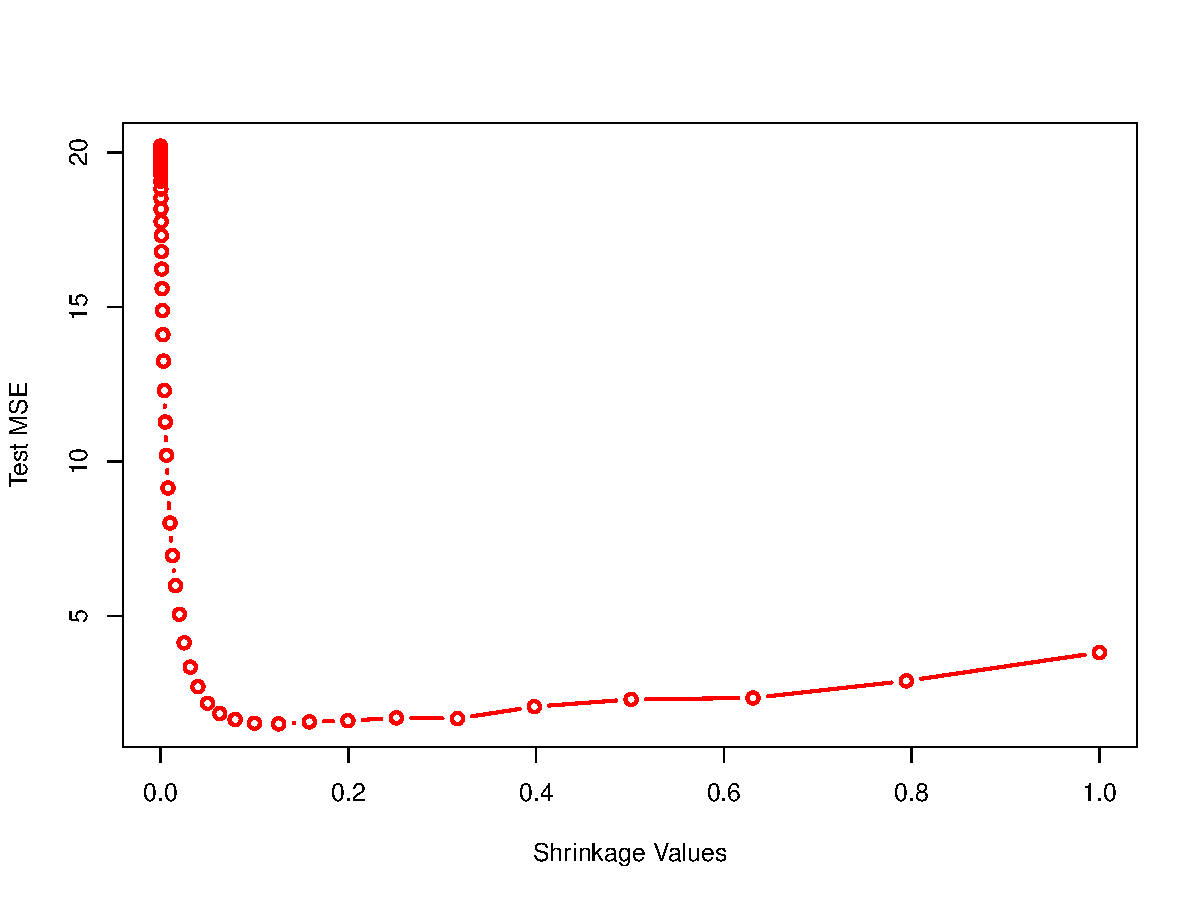
\includegraphics[height=0.5\textheight]{p1.pdf}
\end{center}

\item[\textbf{(e)}] Apply bagging as:

\begin{lstlisting}
library(randomForest)
set.seed(23)
bag.data = randomForest(y~., data=data.train, mtry=40, importance=TRUE)
pred.bag.test = predict(bag.data, newdata=data.test)
bag.test.err = mean((pred.bag.test-y.test)^2)
\end{lstlisting}

Show the test set MSE:

\begin{lstlisting}
bag.test.err 
\end{lstlisting}

\begin{verbatim}
[1] 7.47377

\end{verbatim}

The test set MSE for bagging is $7.47377$.

\item[\textbf{(f)}] Apply random forest to the training set:

\begin{lstlisting}
set.seed(23)
rf.data = randomForest(y~., data=data.train, mtry=13, importance=TRUE)
\end{lstlisting}

For the test set MSE:
\begin{lstlisting}
pred.rf.test = predict(rf.data, newdata=data.test)
rf.test.err = mean((pred.rf.test-y.test)^2)
rf.test.err
\end{lstlisting}

\begin{verbatim}
[1] 7.732766

\end{verbatim}

The test set MSE for the random forest is $7.732766$.

Show importance of the variables:

\begin{lstlisting}
importance(rf.data)
\end{lstlisting}

\begin{verbatim}
         %IncMSE IncNodePurity
x.1  23.87090801     1677.6907
x.2   0.35810518      333.3559
x.3   1.17464376      349.5035
x.4  20.95290681     1475.7868
x.5  -1.34732389      316.3252
x.6  35.68869036     2446.1484
x.7  -1.55473484      316.0630
x.8  54.50399876     4251.4854
x.9   2.81823806      420.5238
x.10  2.85097449      393.0114
x.11 -0.41229165      327.6212
x.12  1.45707758      412.8536
x.13 -0.07614845      330.2071
x.14  1.03408645      378.3150
x.15 72.73041744     5592.5573
x.16  1.53779507      422.7106
x.17 -0.30807860      356.2791
x.18  1.62393917      311.9116
x.19 -1.12441079      326.3051
x.20 16.59394558     1234.1057
x.21  1.51444227      333.4318
x.22  3.52036654      384.4151
x.23  2.35868856      382.6603
x.24 10.09022068      771.6829
x.25 10.68455082      879.2054
x.26  3.75893632      454.7341
x.27 -1.09067523      338.1381
x.28 18.89861330     1383.9493
x.29  0.35818465      321.8541
x.30  3.82742307      401.3689
x.31 -1.15160979      326.7535
x.32 14.29438889      967.1681
x.33 34.71390399     2403.3239
x.34  3.98600438      447.5083
x.35  9.47775240      833.3425
x.36  5.97622152      623.8455
x.37  0.42569931      326.4059
x.38  8.00994315      660.3828
x.39  1.41219689      345.5444
x.40  4.09253787      469.6644
\end{verbatim}

And we can plot them as:

\begin{lstlisting}
varImpPlot(rf.data)
\end{lstlisting}

\begin{center}
	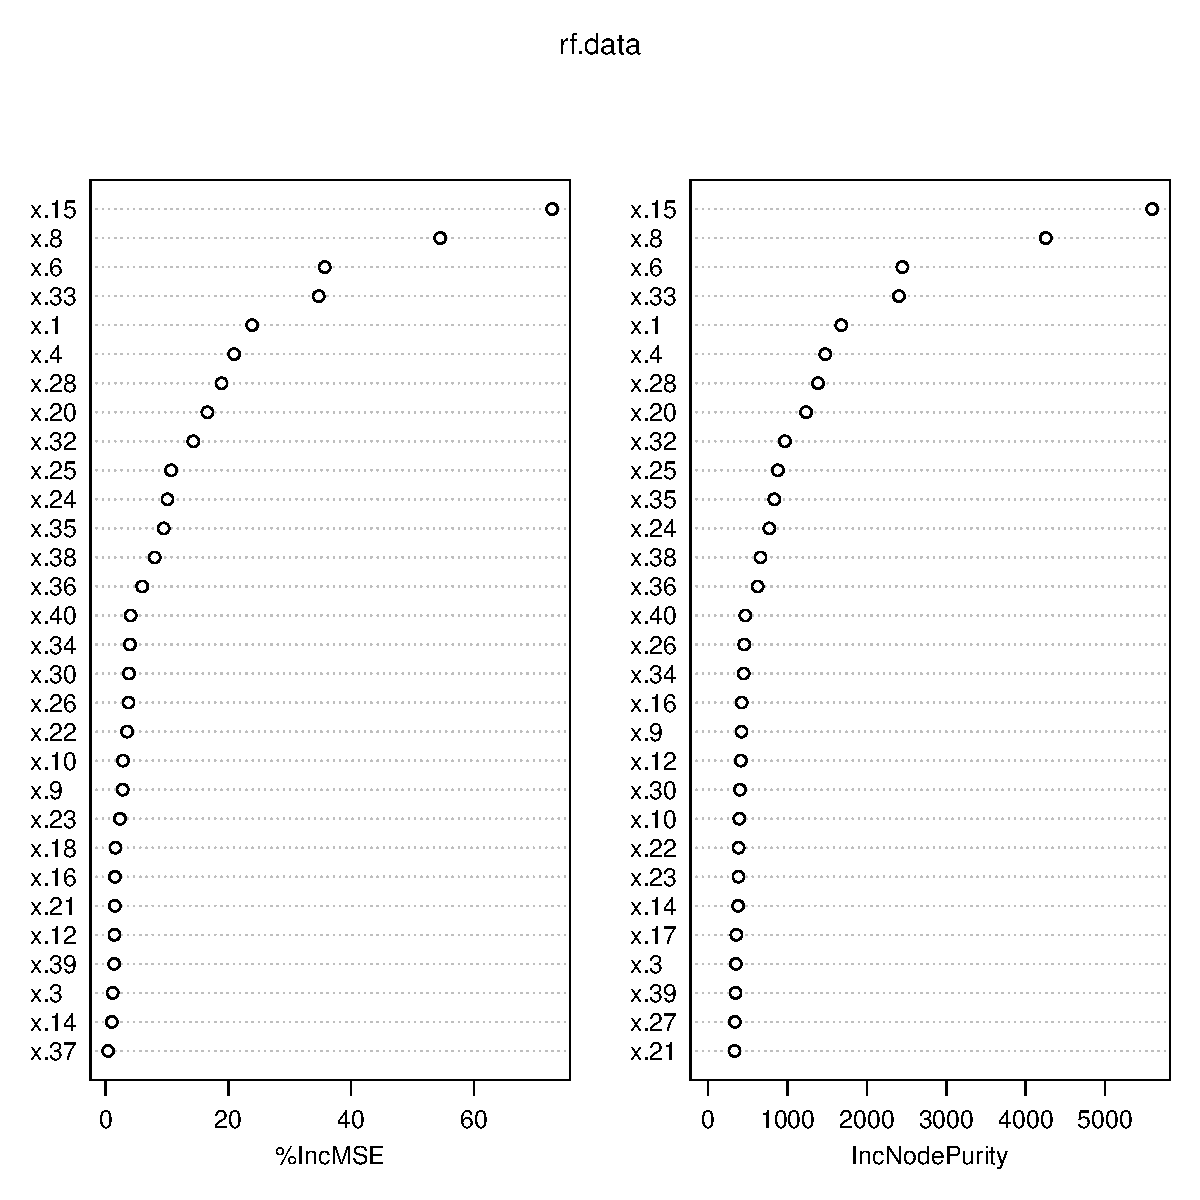
\includegraphics[height=0.6\textheight]{p2.pdf}
\end{center}

Variables x.15 and x.8 appear to be the two most important predictors in the random forest model.

\item[\textbf{(g)}] Perform best subset selection on the training set, plot the training set MSE associated with the best model of each size:

\begin{lstlisting}
library(leaps)
set.seed(23)
regfit.train.err = rep(NA, 40)
regfit.data = regsubsets(y~., data=data.train, nvmax=40)
train.mat = model.matrix(y~., data=data.train, nvmax=40)
for (i in 1:40){
coefi = coef(regfit.data, id=i)
pred.regfit.train = train.mat[, names(coefi)] % * % coefi
regfit.train.err[i] = mean((pred.regfit.train-y.train)^2)
}
plot(regfit.train.err, type="b", col="red", pch=19, lwd=2, xlab="Features in prediction", ylab="Training MSE")
\end{lstlisting}

\begin{center}
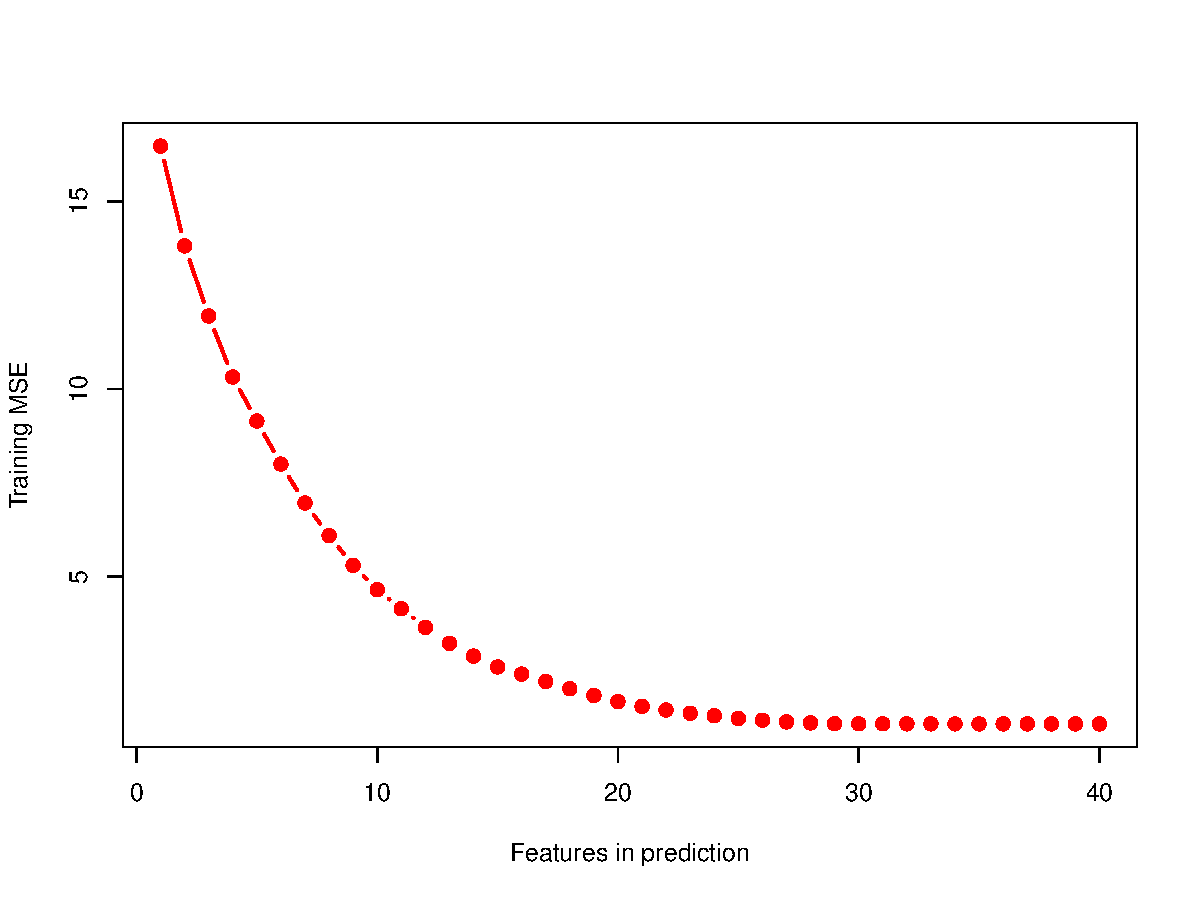
\includegraphics[height=0.5\textheight]{p3.pdf}
\end{center}

\item[\textbf{(h)}] Plot the test set MSE associated with the best model of each size:

\begin{lstlisting}
set.seed(23)
regfit.test.err = rep(NA, 40)
test.mat = model.matrix(y~., data=data.test, nvmax=40)
for (i in 1:40){
coefi = coef(regfit.data, id=i)
pred.regfit.test = test.mat[, names(coefi)] % * % coefi
regfit.test.err[i] = mean((pred.regfit.test-y.test)^2)
}
plot(regfit.test.err, type="b", col="red", pch=19, lwd=2, xlab="Features in prediction", ylab="Test MSE")
\end{lstlisting}

\begin{center}
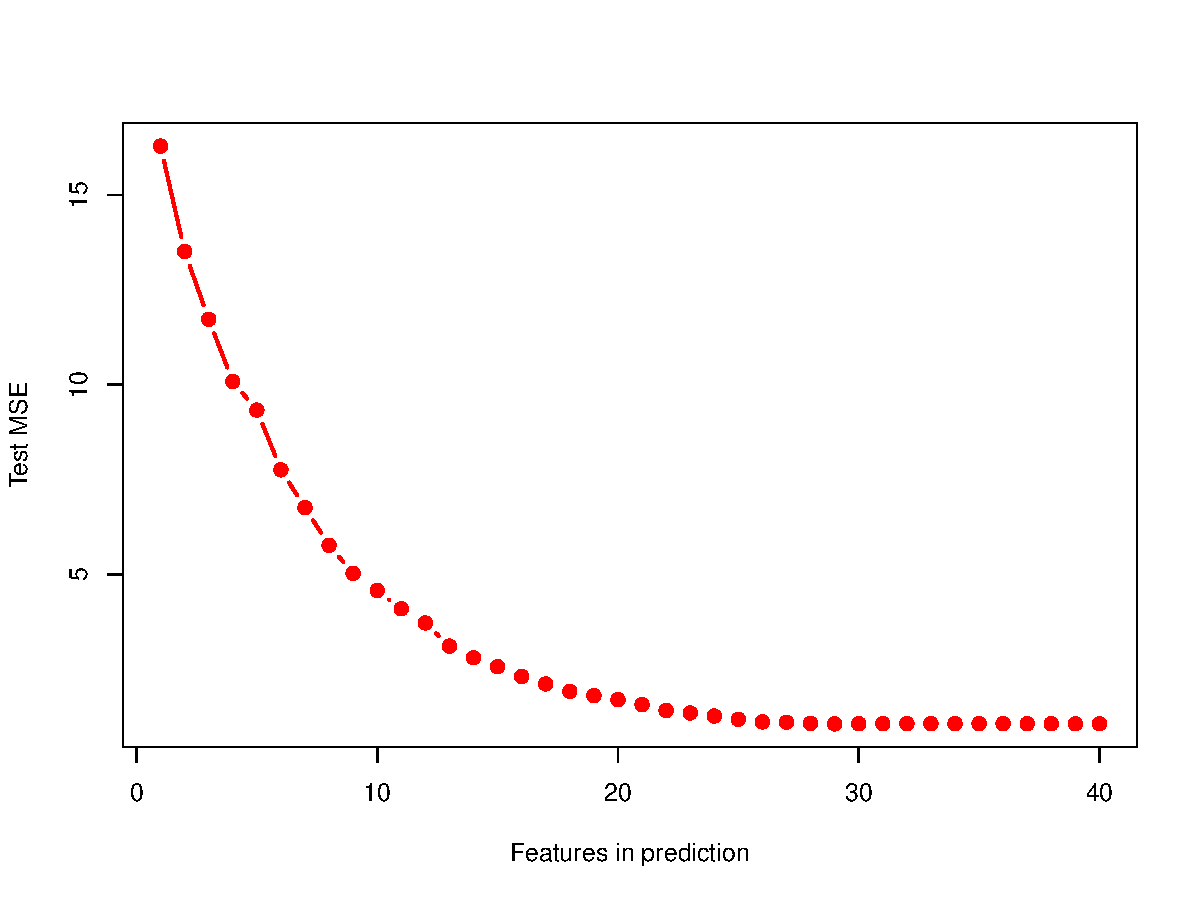
\includegraphics[height=0.5\textheight]{p4.pdf}
\end{center}
 
\item[\textbf{(i)}] Check which model size has the minimum test MSE:

\begin{lstlisting}
which.min(regfit.test.err)
\end{lstlisting}

\begin{verbatim}
[1] 29

\end{verbatim}

So the model with 29 variables has the minimum test MSE.

\item[\textbf{(j)}] Check the coefficient values:

\begin{lstlisting}
coef(regfit.data, id=29)
\end{lstlisting}

\begin{verbatim}
(Intercept)         x.1         x.2 
0.00238244 -1.16720641  0.23645754 
x.3         x.4         x.6 
0.16699470  1.04589096 -1.44426869 
x.8         x.9        x.10 
-1.71070751 -0.32336918 -0.28433311 
x.12        x.14        x.15 
-0.27297398  0.41538162 -2.03644594 
x.16        x.20        x.22 
-0.36922201  1.10242666 -0.26480135 
x.23        x.24        x.25 
0.34663161 -0.73662824 -0.65426426 
x.26        x.27        x.28 
-0.42748998 -0.15248357  0.89620285 
x.30        x.32        x.33 
0.42648698  0.92766354 -1.28265446 
x.34        x.35        x.36 
0.59904794 -0.75540164 -0.49063913 
x.38        x.39        x.40 
-0.72828204 -0.20553657  0.43477006

\end{verbatim}

We can find that all the b elements with value $0$ (b[5], b[7], b[11], b[13], b[17], b[19], b[29], b[31], b[37]) in (a) are not in the best model coefficients.

\item[\textbf{(k)}] Display b errors as:

\begin{lstlisting}
b.err = rep(NA, 20)
x.col = colnames(x, do.NULL=FALSE, prefix="x.")
for (i in 1:40) {
coefi = coef(regfit.data, id=i)
b.err[i] = sqrt(sum((b[x.col %in% names(coefi)]-coefi[names(coefi) %in% x.col])^2) + sum(b[!(x.col %in% names(coefi))])^2)
}
plot(b.err, type="b", col="red", pch=19, lwd=2, xlab="Features in prediction", ylab="beta error")
\end{lstlisting}

The plot is:

\begin{center}
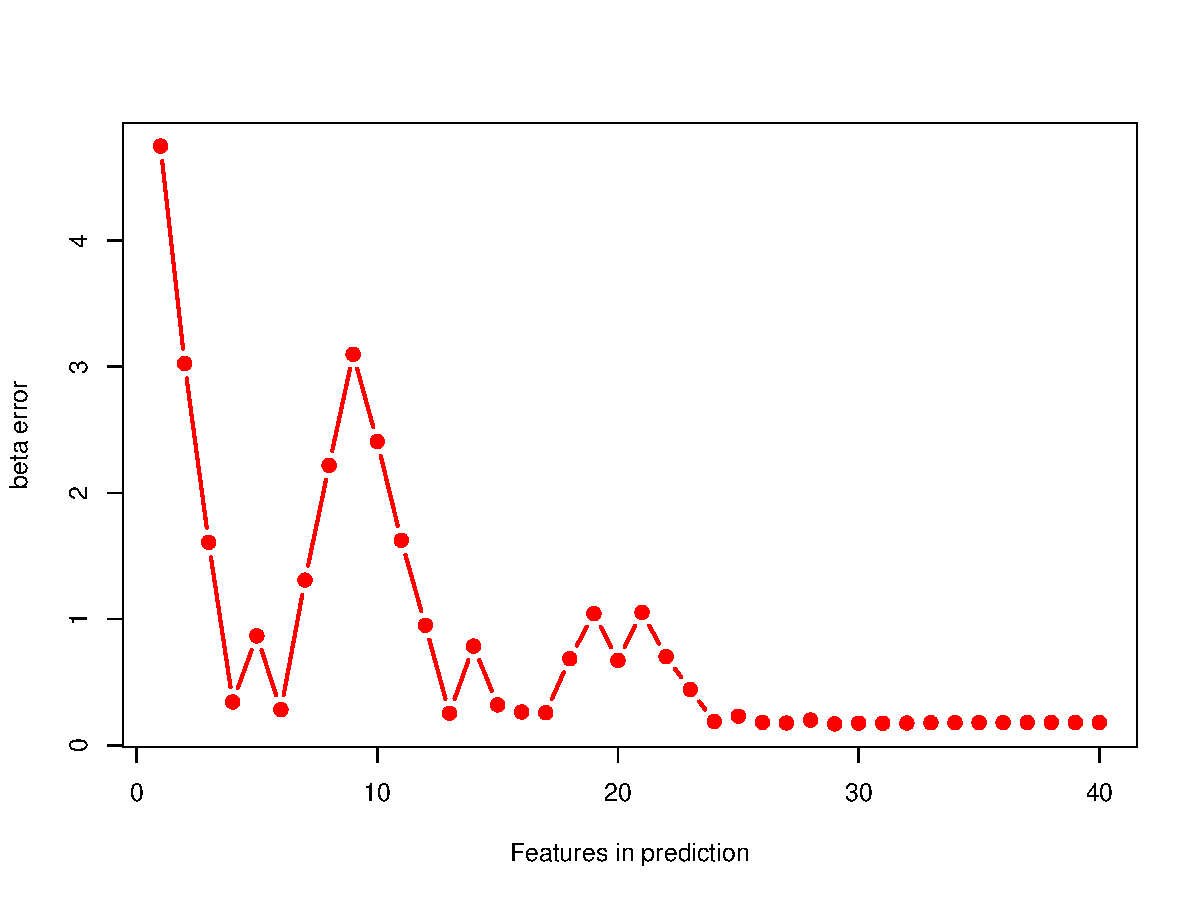
\includegraphics[height=0.5\textheight]{p5.pdf}
\end{center}

We can have the minimum error between the estimated and true coefficients at:

\begin{lstlisting}
which.min(b.err)
\end{lstlisting}

\begin{verbatim}
[1] 29

\end{verbatim}

So in this particular case, both the test error and the error between the estimated and true coefficients are at the model with 29 variables.

\item[\textbf{(l)}] Show the table as:

\begin{lstlisting}
table.errs = matrix(c(boost.test.err[which.min(boost.test.err)], bag.test.err, rf.test.err, regfit.test.err[which.min(regfit.test.err)]), ncol=4, byrow=TRUE)
colnames(table.errs) = c("Boosting", "Bagging", "Random Forest", "Model Selection")
rownames(table.errs) = c("MSE")
table.errs
\end{lstlisting}

\begin{lstlisting}
    Boosting Bagging Random Forests Model Selection
MSE 1.511832 7.47377       7.732766        1.058832
\end{lstlisting}

In this case, model selection by exhaustive search using the regsubsets() function has the minimum MSE. It maybe because some elements of b are intended for zero, so by model selection, these zero variables are neglected in the model, the errors of these useless variables are prevented from the model, so we have the minimum MSE by the best subset selection.

\end{enumerate}



\section*{Problem 2}
Given a two data points data set, one from each class, such that:
\begin{align*}
\vect{x_1} \in \mathcal{C}^+ (t_1=+1)\\
\vect{x_2} \in \mathcal{C}^- (t_1=-1)
\end{align*}

In order to maximize margin, there exist two constraints:

\begin{align}
\vect{w}^\mathrm{T} \vect{x_1} + b - 1 = 0 \\
\vect{w}^\mathrm{T} \vect{x_2} + b + 1 = 0
\end{align}

Denote $\lambda_1$ and $\lambda_2$ be the Lagrange multipliers, we can have the following Lagrange function:

\begin{align*}
L(\vect{w}, b, \lambda) = \frac{1}{2} \lVert \vect{w} \rVert^2 - \lambda_1 (\vect{w}^\mathrm{T} \vect{x_1} + b -1) - \lambda_2 (\vect{w}^\mathrm{T} \vect{x_2} + b +1)
\end{align*}

Setting the derivatives of $L(\vect{w}, b, \lambda)$ with respect to $\vect{w}$ and $b$ equal to zero:
\begin{align}
\frac{\partial L(\vect{w}, b, \lambda)  }{\partial \vect{w}} 
&=\vect{w} - \lambda_1 \vect{x_1} - \lambda_2 \vect{x_2}
= 0\\
\frac{\partial L(\vect{w}, b, \lambda)  }{\partial b} 
&= - \lambda_1 -  \lambda_2
= 0
\end{align}

By equation \textbf{(4)}, we have:
\begin{align}
\lambda_2 = -\lambda_1
\end{align}

Substitute \textbf{(5)} in equation \textbf{(3)}, we have:
\begin{align}
\vect{w} = \lambda_1(\vect{x_1} - \vect{x_2})
\end{align}

By equation \textbf{(1)} and \textbf{(2)}, and substitute $\vect{w}$, we have:
\begin{align*}
b 
&= -\frac{1}{2} \vect{w}^\mathrm{T} (\vect{x_1} + \vect{x_2})\\
&=  -\frac{\lambda_1}{2} (\vect{x_1} - \vect{x_2})^\mathrm{T} (\vect{x_1} + \vect{x_2})\\
&=  -\frac{\lambda_1}{2} (\vect{x_1}^\mathrm{T} - \vect{x_2}^\mathrm{T}) (\vect{x_1} + \vect{x_2})\\
&=  -\frac{\lambda_1}{2} (\vect{x_1}^\mathrm{T}\vect{x_1} - \vect{x_2}^\mathrm{T}\vect{x_2})
\end{align*}

The values of $\vect{w}$ and $b$ have demonstrate that, irrespective of the dimensionality of the data space, a two data points data set, one from each class, is sufficient to determine the location of the maximum-margin hyperplane.


\section*{Problem 3}
By the exponential error function, we have:

\begin{align*}
\mathbb{E}_{\vect{x},t} [\exp\{-ty(\vect{x})\}] = \sum_t \int \exp\{ -ty(\vect{x})\}p(t | \vect{x})p(\vect{x}) \mathrm{d}\vect{x}
\end{align*}

Perform a variational minimization with respect to all possible functions y(x), we obtain:

$$
y(\vect{x}) = \frac{1}{2} \ln \left\{ \frac{p(t=+1| \vect{x} )}{p(t=-1| \vect{x} )} \right\} 
$$

That is:
$$
p(t=\pm 1| \vect{x}) = \frac{1}{1+ e^{-2y(\vect{x})}}
$$

Using a log likelihood of logistic regression model, which is well-behaved probabilistic model, on the $p(t| \vect{x})$, then we need to minimize $$\ln (1+e^{-2\theta})$$
 
While, by definition, the Adaboost minimizes the average of $$e^{-\theta}$$

Because $\ln (1+e^{-2\theta})$ is bounded to linear growth, while $e^{-\theta}$ is bounded to exponential growth. This has demonstrated that the corresponding conditional distribution $p(t| \vect{x})$ cannot be correctly normalized. So the above exponential error function, which is minimized by the AdaBoost algorithm, does not correspond to the log likelihood of any well-behaved probabilistic model.


\end{document} 
